\section{Program til skalaer}
\label{TestAfSkalaProgramSkala}
%
Programmet som blev brugt til at præsentere skalaerne for deltagerne blev udviklet i Processing 3.3.6. De bygger på et widget-bibliotek lavet af Søren Krarup Olesen m.fl. som hedder PDPGUITest. I programmet er der lavet classes til blandt andet check boxes, radio buttons, sliders og lignende GUI elementer, som kan interageres med og som kan gemme data fra besvarelserne. 

I setup konstrueres objekter fra klasserne PDPGUI, PDPPushButton og PDPVASknapper. Heri defineres tekst, størrelse og placering af knapper. Det er også her hvor spørgsmål og labels på skalaerne defineres.
Der laves også en tabel, med en navngivet kolonne og til hvert datapunkt.

I draw-loopet er der 7 forskellige skærmbilleder som præsenteres for deltagerne. Skærmbillederne dannes ved at loade de widgets ind som blev konstruerede i setuppet, se linje 154 og 160-164 på \autoref{fig:Screen}. For de bipolare skalaer som har en markering af midten, er en linje tilføjet oven på den pågældende widget, se linje 157-159. Det samme gælder i de tilfælde hvor der er et label på midterpunktet. 
Hvert skærmbillede loades med variablen ``screen'', som starter med at være 1. Når der trykkes på ``Næste'', øges ``screen'' med 1, hvilket gør det næste if-statement sandt og dermed skifter til næste skærmbillede. Logikken bag tilbage-knappen er den samme, bortset fra at ``screen'' mindskes med 1 når der trykkes på ``Tilbage''. Den del af koden som er ansvarlig for navigationen mellem siderne kan ses på \autoref{fig:Screen}, hvor linje 153 og 181 tjekker hvilket skærmbillede der skal vises, linje 165 og 173 øger ``screen'' så den går videre til næste skærmbillede og linje 176 og 177 mindsker ``screen'', så den går videre til forrige skærmbillede.
``Næste'' knappen gør også at det indtastede data gemmes i datatabellen, hvilket kan ses i linje 166-172. Linje 174 og 178 fjerner de eksisterende widgets fra skærmbilledet, når der skiftes til henholdsvis næste eller forrige skærm.
\begin{figure}[H]
\centering
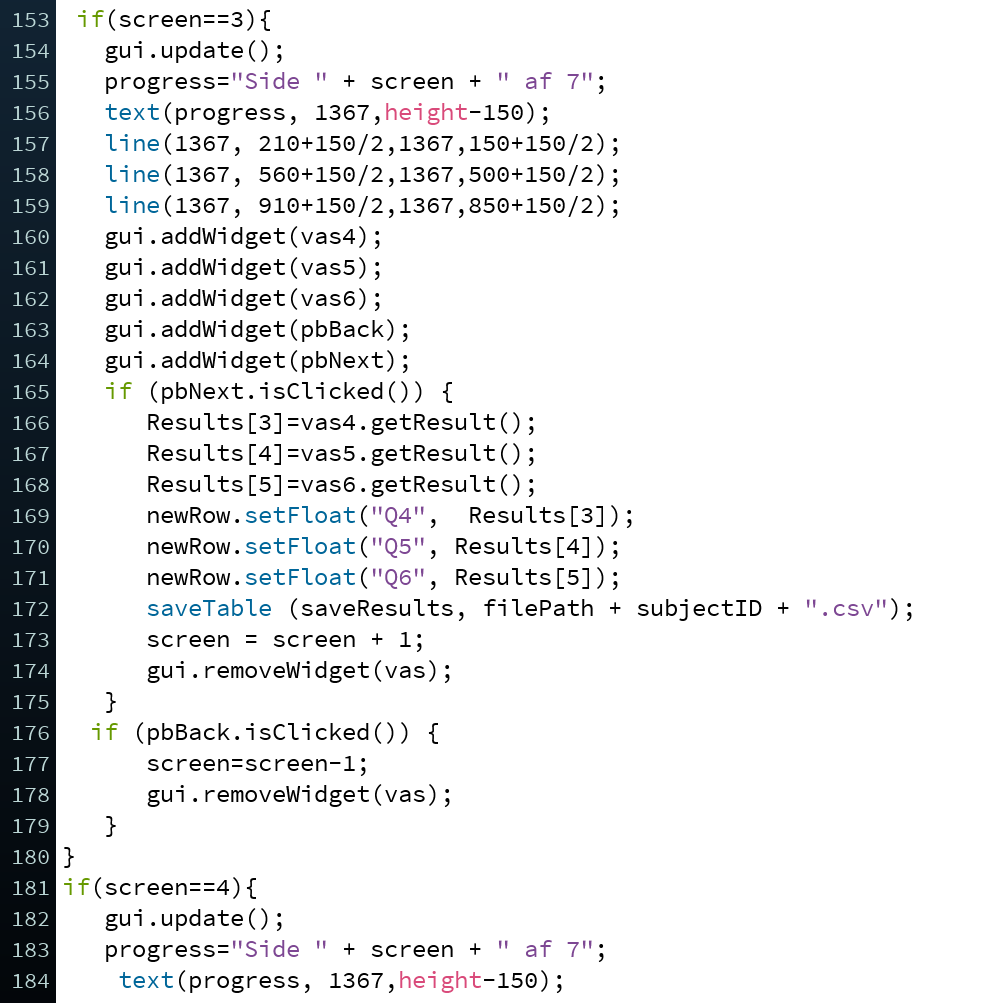
\includegraphics[width =0.7\textwidth]{Figure/VASProgram/Screen} 
\caption{Udpluk af koden, som viser hvordan et skærmbillede er sættes op og hvordan der navigeres mellem forskellige skærmbilleder.}
\label{fig:Screen}
\end{figure}
\noindent
%
Samme fremgangsmåde er anvendt til de alle skærmbilleder med skalaer. Når der trykkes ``Næste'' på det sidste skærmbillede med skalaer, skiftes til en side hvor der står ``Tak for hjælpen'', se linje 304-308 på \autoref{fig:Tak}.
\begin{figure}[H]
\centering
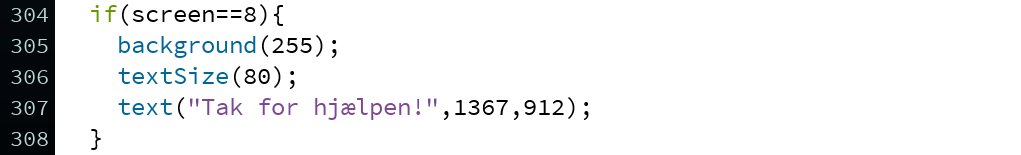
\includegraphics[width =0.7\textwidth]{Figure/VASProgram/Tak} 
\caption{Udpluk af koden, som viser hvordan et skærmbillede er sættes op og hvordan der navigeres mellem forskellige skærmbilleder.}
\label{fig:Tak}
\end{figure}
\noindent
%

Programmet bærer kraftigt præg af at det blev lavet i sidste øjeblik, da der var en fastsat aftale med lufthavnen i forhold til hvornår testen skulle udføres. Det havde derfor nogle fejl og mangler, som med fordel kan udbedres til en anden gang. Herunder opsummeres de problemer som blev opdaget og eventuelle løsningsforslag til hvordan man kan optimere bruget 

Man kan gå videre uden at vælge noget. Kan løses ved at tjekke om data er gemt for skalaerne på det nuværende skærmbillede og bruge det som en betingelse for at ``screen'' kan øges med 1.

Den skriver 0 når der ikke bliver valgt noget. Ved at løse problemet med at folk gik videre uden at svare, forsvinder dette problem også, da der aldrig vil være ubesvarede skalaer. Alternativt kan det vælges at skrive ``NaN'', hvis ikke brugeren har valgt noget.

Den reagerer dårligt på tryk. Problemet skyldes sandsynligvis at programmet er en smule ineffektivt og bruger meget processorkraft på at læse kode som ikke bruges på det pågældende skærmbillede. For at optimere det, kan man med fordel lave en PDPGUI for hvert skærmbillede, frem for at slette de gamle widgets og loade de nye hver gang. Man burde også bruge while-loops for hvert skærmbillede, frem for if-statements, så computeren ikke skal gennem hele koden i hver iteration, men kun skal læse den kode som bruges på det tilstedeværende skærmbillede.

Programmet fremgår af \fullref{ElektroniskBilagProgram}.
